\section{Введение}
\begin{figure}[htbp]
    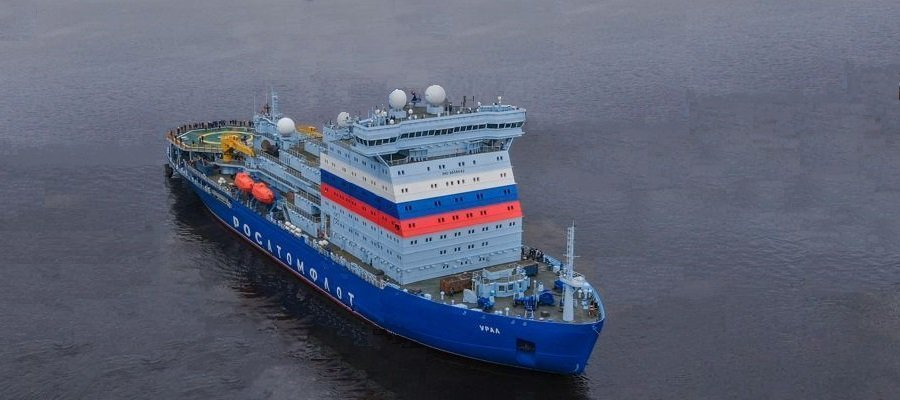
\includegraphics[scale=0.5]{src/Introduction/assets/Ледокол.jpg}
\caption{Ледокол Урал}\label{fig:IceBreker}
\end{figure}
Развитие судоходства в Арктике требует создания и внедрения современных технологических решений для обеспечения безопасности и 
эффективности морских операций. Ледоколы играют ключевую роль в освоении этих регионов, обеспечивая проход судов через ледовые поля и выполняя различные 
научно-исследовательские и промышленные задачи. Бортовой измерительный комплекс (БИК) должен стать важной частью ледокола, поскольку позволит автоматизировать часть работы
команды судна, что позволит исследователям больше заниматься анализом данных, нежели их сбором.

Сейчас анализ ледовой обстановки выполняется человеком. Специалисту приходится при помощи камер выглядывать за борт судна, чтобы оценить толщину ледового
покрытия, самостоятельно наблюдать за эволюцией ледового канала, который оставляет за собой ледокол. БИК призван  исправить эту ситуацию, 
автоматизировав сбор информации о ледовой обстановке около ледокола.

Комплекс, разработка части которого была положена в основу данной работы, в течение зимы 2023--2024 годов и весны 2024 года был установлен на борту ледокола Урал и
тестировался всё это время.

В настоящей работе описаны результаты разработки алгоритмов для обработки изображения ледового канала. Была проанализирована литература и рассмотрены
различные подходы. Результатом работы стали два алгоритма по построению масок. Первый основан на EM алгоритме для попиксельной сегментации, он был разработан в очень сжатые сроки,
чтобы как можно раньше начать собирать данные. Второй алгоритм уже использует нейросетевой подход, основанный на бэкбоуне, обучавшемся на задаче решения пазлов, и дополненный 
предобученным трансформером с архитектурой DINO для уточнения меток. В работе представлены как описания этих алгоритмов, так и полученные результаты. 